\documentclass[pdflatex,compress,mathserif]{beamer}

%\usetheme[dark,framenumber,totalframenumber]{ElektroITK}
\usetheme[darktitle,framenumber,totalframenumber]{ElektroITK}

\usepackage[utf8]{inputenc}
\usepackage[T1]{fontenc}
\usepackage{lmodern}
\usepackage[english]{babel}
\usepackage{amsmath}
\usepackage{amsfonts}
\usepackage{amssymb}
\usepackage{graphicx}
\usepackage{multicol}
\usepackage{lipsum}
\usepackage{framed}
\usepackage{minted}

\definecolor{LightGray}{gray}{0.95}

\usefonttheme[onlymath]{serif}

\newcommand*{\Scale}[2][4]{\scalebox{#1}{$#2$}}%

\setbeamertemplate{caption}[numbered]

\title{Digital Signal Processing}
\subtitle{Discrete Fourier Transform (DFT)}

\author{Mifta Nur Farid}
\date{August $\text{21}^\text{st}$, 2023}

\begin{document}

\maketitle

\section{Discrete Fourier Transform}

\begin{frame}{Discrete Fourier Transform}
    \begin{itemize}
        \item The signal frequency content is very useful than the digital signal samples (Fig. \ref{fig:04.01})
        \item Discrete Fourier Transform (DFT): the algorithm transforming the time domain signal samples to the frequency domain components
        
    \end{itemize}
\end{frame}

\begin{frame}{Discrete Fourier Transform}
    \begin{figure}
        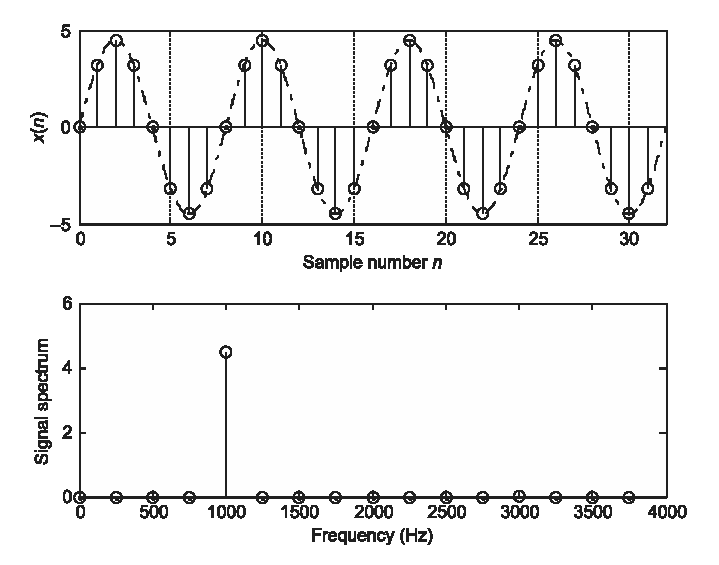
\includegraphics[width=0.7\linewidth]{fig/fig.4.01}
        \caption{Example of the digital signal and its amplitude spectrum.}
        \label{fig:04.01}
    \end{figure}
\end{frame}

\subsection{Fourier Series Coefficients of Periodic Digital Signals}

\begin{frame}{Fourier Series Coefficients of Periodic Digital Signals}
    \begin{itemize}
        \item Periodic digital signal $x(n)$ sampled at a rate $f_s$ Hz with fundamental period $T_0 = NT$ (Fig. \ref{fig:04.02})
    \end{itemize}
    \begin{figure}
        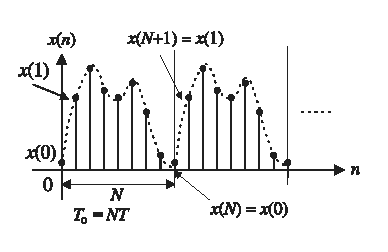
\includegraphics[width=0.6\linewidth]{fig/fig.4.02}
        \caption{Periodic digital signal.}
        \label{fig:04.02}
    \end{figure}
\end{frame}

\begin{frame}{Fourier Series Coefficients of Periodic Digital Signals}
    \begin{itemize}
        \item The coefficients of the Fourier series expansion of the periodic signal $x(t)$ in a complex form is
        \begin{equation}
            c_k=\frac{1}{T_0} \int_{T_0}x(t)e^{-jk\omega_0 t} dt,~~-\infty<k<\infty
        \end{equation}
        \item $k$ is the number of harmonics corresponding to the harmonic frequency of $kf_0$
        \item $\omega_0 = 2\pi/T_0$ and $f_0 = 1/T_0$ are the fundamental frequency.
    \end{itemize}
\end{frame}

\begin{frame}{Fourier Series Coefficients of Periodic Digital Signals}
    \begin{itemize}
        \item we substitute $T_0=NT$, $\omega_0=2\pi/T_0$ and approximate the integration over one period using a summation by substituting $dt=T$ and $t=nT$
        \begin{equation}
            c_k=\frac{1}{N} \sum_{n}^{N-1}x(n)e^{-j2\pi k n/N},~~-\infty<k<\infty
        \end{equation}
        \item $c_k$: discrete-time Fourier series coefficients
    \end{itemize}
\end{frame}

\begin{frame}{Fourier Series Coefficients of Periodic Digital Signals}
    \begin{itemize}
        \item discrete-time Fourier series coefficients $c_k$ is periodic of $N$
        \item proof:
        \begin{equation}
            \begin{aligned}[b]
                c_{k+N} &= \frac{1}{N} \sum_{n}^{N-1}x(n)e^{-j2\pi (k+N) n/N} \\
                &= \frac{1}{N} \sum_{n}^{N-1}x(n)e^{-j2\pi k n/N} e^{-j2\pi n}
            \end{aligned}
        \end{equation}
        \item $e^{-j2\pi n} = \cos(2\pi n) - j\sin(2 \pi n) = 1$, then
        \begin{equation}
            c_{k+N} = c_k
            \label{eq:4.4}
        \end{equation}
    \end{itemize}
\end{frame}

\begin{frame}{Fourier Series Coefficients of Periodic Digital Signals}
    \begin{itemize}
        \item Therefore, the two-sided line amplitude spectrum $|c_k|$ is periodic
        \begin{figure}
            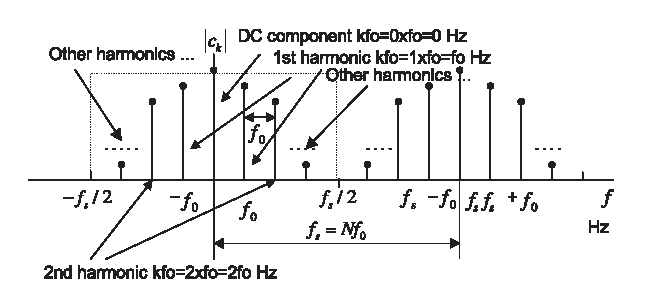
\includegraphics[width=\linewidth]{fig/fig.4.03}
            \caption{Amplitude spectrum of the periodic digital signal..}
            \label{fig:04.03}
        \end{figure}
    \end{itemize}
\end{frame}

\begin{frame}{Fourier Series Coefficients of Periodic Digital Signals}
    Note for Fig. \ref{fig:04.03}
    \begin{enumerate}
        \item only the line spectral portion between the frequencies $-f_s/2$ and $f_s/2$ (nyquist frequency) represents frequency information of the periodic signal.
    \end{enumerate}
\end{frame}

\begin{frame}{Fourier Series Coefficients of Periodic Digital Signals}
    \begin{enumerate}\setcounter{enumi}{1}
        \item the spectral portion from $f_s/2$ to $f_s$ is a copy of the spectrum in the negative frequency range from $-f_s/2$ to 0 Hz due to the spectrum being periodic for every $Nf_0$ Hz.\\ For convenience, we compute the spectrum over the range from 0 to $f_s$ Hz with nonnegative indices, that is,
        \begin{equation}
            c_k=\frac{1}{N} \sum_{n=0}^{N-1}x(n)e^{-j2\pi k n/N},~~k=0,1,\cdots,N-1
            \label{eq:4.5}
        \end{equation}
        We can apply Eq. (\ref{eq:4.4}) to find the negative indexed spectral values if they are required
    \end{enumerate}
\end{frame}

\begin{frame}{Fourier Series Coefficients of Periodic Digital Signals}
    \begin{enumerate}\setcounter{enumi}{2}
        \item For the $k$-th harmonic, the frequency is
        \begin{equation}
            f = kf_0 \text{ Hz}
        \end{equation}
        The frequency spacing between the consecutive spectral lines, called the frequency resolution, is $f_0$ Hz.
    \end{enumerate}
\end{frame}

\subsection{Discrete Fourier Transform}

\begin{frame}{Discrete Fourier Transform}
    \begin{itemize}
        \item we assume that the process acquires data samples from digitizing the interested continuous signal for a duration of $T_0$ seconds.
    \end{itemize}
    \begin{figure}
        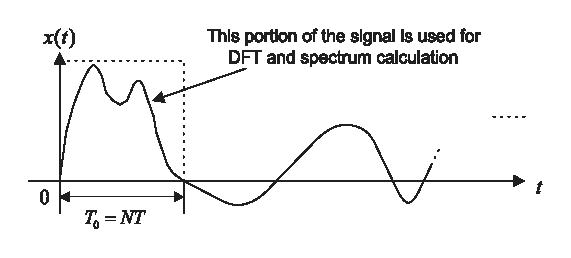
\includegraphics[width=\linewidth]{fig/fig.4.06a}
    \end{figure}
\end{frame}

\begin{frame}{Discrete Fourier Transform}
    \begin{itemize}
        \item a periodic signal $x(n)$ is obtained by copying the acquired $N$ data samples with the duration of $T_0$ to itself repetitively
    \end{itemize}
    \begin{figure}
        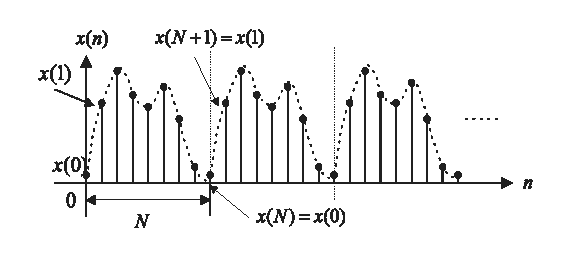
\includegraphics[width=\linewidth]{fig/fig.4.06b}
    \end{figure}
\end{frame}

\begin{frame}{Discrete Fourier Transform}
    \begin{itemize}
        \item we determine the Fourier series coefficients using one-period $N$ data samples
        and Eq. (\ref{eq:4.5}).
        \item Then we multiply the Fourier series coefficients by a factor of $N$ to obtain
        \begin{equation}
            \begin{aligned}[b]
                X(k) &= Nc_k \\
                &= \sum_{n=0}^{N-1} x(n)e^{-j2\pi kn / N},\text{ for } k = 0,1, \cdots, N-1
            \end{aligned}
        \end{equation}
        where $X(k)$ constitutes the DFT coefficients
    \end{itemize}
\end{frame}

\begin{frame}{Discrete Fourier Transform}
    \begin{figure}
        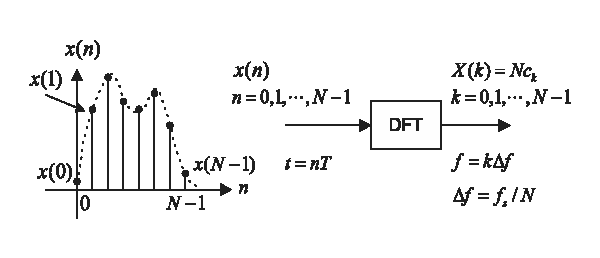
\includegraphics[width=\linewidth]{fig/fig.4.06c}
    \end{figure}
\end{frame}

\begin{frame}{Discrete Fourier Transform}
    DFT definition:
    \begin{equation}
        \begin{aligned}[b]
            X(k) &= \sum_{n=0}^{N-1} x(n)e^{-j2\pi kn / N},\text{ for } k = 0,1, \cdots, N-1 \\
            X(k) &= \sum_{n=0}^{N-1} x(n)W_N^{kn},\text{ for } k = 0,1, \cdots, N-1 \\
        \end{aligned}
        \label{eq:4.8}
    \end{equation}
    \begin{equation}
        \begin{aligned}[b]
            X(k) &= x(0)W_N^{k0} + x(1)W_N^{k1} + x(2)W_N^{k2} + \cdots \\
            &+ x(N-1)W_N^{k(N-1)},\text{ for } k = 0,1, \cdots, N-1 \\
        \end{aligned}
        \label{eq:4.9}
    \end{equation}
    $W_N$ is the twiddle factor
    \begin{equation}
        W_N = e^{-j2\pi /N} = \cos(\frac{2\pi}{N}) - j\sin(\frac{2\pi}{N})
    \end{equation}
\end{frame}

\begin{frame}{Discrete Fourier Transform}
    \begin{itemize}
        \item To determine the inverse of DFT (IDFT), we can multiply both sides of Eq. (\ref{eq:4.8}) by $e^{j2 \pi k m /N}$ and sum from $k = 0$ to $k = N - 1$, that is
        
        \begin{equation}
            \begin{aligned}[b]
                \sum_{k=0}^{N-1} X(k)e^{j\frac{2\pi km}{N}} &= \sum_{k=0}^{N-1} \sum_{k=0}^{N-1} x(n)e^{-j\frac{2\pi kn}{N}}e^{j\frac{2\pi km}{N}} \\
                &= \sum_{n=0}^{N-1} x(n) \sum_{n=0}^{N-1} e^{j\frac{2\pi k(m-n)}{N}}
            \end{aligned}
            \label{eq:4.11}
        \end{equation}
        note that
        \begin{equation}
            \sum_{n=0}^{N-1} e^{j\frac{2\pi k(m-n)}{N}} = \begin{cases}
                N,& m = n\\
                0,& m \neq n
            \end{cases}
        \end{equation}
    \end{itemize}
\end{frame}


\begin{frame}{Discrete Fourier Transform}
    \begin{itemize}
        \item Thus, Eq. (\ref{eq:4.11}) becomes
        \begin{equation}
            \sum_{k=0}^{N-1} X(k)e^{j\frac{2\pi km}{N}} = \sum_{n=0}^{N-1} x(n) \sum_{k=0}^{N-1} e^{j\frac{2\pi k(m-n)}{N}}
            \label{eq:4.14}
        \end{equation}
    \end{itemize}
\end{frame}

\begin{frame}{Discrete Fourier Transform}
    \begin{itemize}
        \item Using Eq. (\ref{eq:4.14}), we see that
    \end{itemize}
    \begin{align*}
        \text{for } m = 0,~\sum_{k=0}^{N-1} X(k)e^{j\frac{2\pi k0}{N}} &= \sum_{n=0}^{N-1} x(n) \sum_{k=0}^{N-1} e^{j\frac{2\pi k(0-n)}{N}} \\
        &= x(0)\sum_{k=0}^{N-1}1 = Nx(0) \\
        \text{for } m = 1,~\sum_{k=0}^{N-1} X(k)e^{j\frac{2\pi k1}{N}} &= \sum_{n=0}^{N-1} x(n) \sum_{k=0}^{N-1} e^{j\frac{2\pi k(1-n)}{N}} \\
        &= x(1)\sum_{k=0}^{N-1}1 = Nx(1) \\
    \end{align*}
\end{frame}

\begin{frame}{Discrete Fourier Transform}
    \begin{align*}
        \vdots\\
        \text{for } m = N-1,~\sum_{k=0}^{N-1} X(k)e^{j\frac{2\pi k(N-1)}{N}} &= \sum_{n=0}^{N-1} x(n) \sum_{k=0}^{N-1} e^{j\frac{2\pi k(N-1-n)}{N}} \\
        &= x(N-1)\sum_{k=0}^{N-1}1 = Nx(N-1) \\
    \end{align*}
\end{frame}

\begin{frame}{Discrete Fourier Transform}
    \begin{itemize}
        \item As a summary, we conclude
        \begin{equation}
            x(m) = \frac{1}{N} \sum_{k=0}^{N-1} X(k) e^{j\frac{2 \pi km}{N}}
        \end{equation}
        \item The inverse of DFT is given by
        \begin{equation}
            \begin{aligned}[b]
                x(n) &= \frac{1}{N} \sum_{k=0}^{N-1} X(k) e^{j\frac{2 \pi km}{N}} \\
                &= \frac{1}{N} \sum_{k=0}^{N-1} X(k) W_N^{-kn}, \text{ for } n=0,1,\cdots,N-1
            \end{aligned}
            \label{eq:4.15}
        \end{equation}
    \end{itemize}
\end{frame}

\begin{frame}{Discrete Fourier Transform}
    \begin{itemize}
        \item Similar to Eq. (\ref{eq:4.8}), the expansion of Eq. (\ref{eq:4.15}) leads to
        \begin{equation}
            \begin{aligned}[b]
                x(n) =& \frac{1}{N} \left( X(0)  W_N^{-0n} + X(1) W_N^{-1n} + X(2) W_N^{-2n} \right.\\
                & + \cdots + X(N-1) \left. W_N^{-(N-1)n} \right) \text{,} \\
                & \text{ for } n=0,1,\cdots,N-1
            \end{aligned}
        \end{equation}
        \item In time domain we use the sample number or time index $n$ for indexing the digital sample sequence $x(n)$.
        \item However, in frequency domain, we use index $k$ for indexing $N$ calculated DFT coefficients $X(k)$.
        \item We also refer $k$ as the frequency bin number in Eq. (\ref{eq:4.8}) and Eq. (\ref{eq:4.9})
    \end{itemize}
\end{frame}

\begin{frame}[fragile]{Discrete Fourier Transform}
    \begin{itemize}
        \item We can do DFT and inverse DFT in python:
    \end{itemize}
    \begin{minted}[frame=lines,framesep=2mm,fontsize=\small,bgcolor=LightGray]{python}
from scipy.fft import fft
from scipy.io import wavfile

# x = input vector
samplerate, x = wavfile.read('audio.wav')

# calculate DFT coefficients
X = fft.fft(x) # X = DFT coefficient vector

# inverse of DFT
x = fft.ifft(X)
    \end{minted}
\end{frame}

\begin{frame}[fragile]{Discrete Fourier Transform}
    \textbf{Example:}
    \begin{itemize}
        \item Given a sequence $x(n)$ for $0 \leq n \leq 3$, where $x(0) = 1$, $x(1) = 2$, $x(2) = 3$, and $x(3) = 4$, evaluate its DFT $X(k)$.
    \end{itemize}
\end{frame}

\begin{frame}[fragile]{Discrete Fourier Transform}
    \textbf{Solution:}
    \begin{itemize}
        \item Since $N = 4$ and $W_4 = e^{-j\frac{\pi}{2}}$, using Eq. (\ref{eq:4.8}) we have a simplified formula
        \begin{equation*}
            X(k) = \sum_{n=0}^{3} x(n) W_{4}^{kn} = \sum_{n=0}^{3} x(n)e^{-j\frac{\pi kn}{2}},\text{ for } k = 0,1,2,3
        \end{equation*}
    \end{itemize}
\end{frame}

\begin{frame}[fragile]{Discrete Fourier Transform}
    \textbf{Solution (cont.):}
    \begin{itemize}
        \item For $k = 0$
        \begin{align*}
            X(0) &= \sum_{n=0}^{3} x(n)e^{-j\frac{\pi 0n}{2}} \\
            &= x(0)e^{-j0} + x(1)e^{-j0} + x(2)e^{-j0} + x(3)e^{-j0} \\
            &= x(0) + x(1) + x(2) + x(3) \\
            &= 1 + 2 + 3 + 4 \\
            X(0) &= 10
        \end{align*}
    \end{itemize}
\end{frame}

\begin{frame}[fragile]{Discrete Fourier Transform}
    \textbf{Solution (cont.):}
    \begin{itemize}
        \item For $k = 1$
        \begin{align*}
            X(1) &= \sum_{n=0}^{3} x(n)e^{-j\frac{\pi n}{2}} \\
            &= x(0)e^{-j0} + x(1)e^{-j\frac{\pi}{2}} + x(2)e^{-j \pi} + x(3)e^{-j\frac{3\pi}{2}} \\
            &= x(0) - jx(1) - x(2) + jx(3) \\
            &= 1 - j2 - 3 + j4 \\
            X(1) &= -2 + j2
        \end{align*}
    \end{itemize}
\end{frame}

\begin{frame}[fragile]{Discrete Fourier Transform}
    \textbf{Solution (cont.):}
    \begin{itemize}
        \item For $k = 2$
        \begin{align*}
            X(2) &= \sum_{n=0}^{3} x(n)e^{-j \pi n} \\
            &= x(0)e^{-j0} + x(1)e^{-j\pi} + x(2)e^{-j2\pi} + x(3)e^{-j3\pi} \\
            &= x(0) - x(1) + x(2) - x(3) \\
            &= 1 - 2 + 3 - 4 \\
            X(2) &= -2
        \end{align*}
    \end{itemize}
\end{frame}

\begin{frame}[fragile]{Discrete Fourier Transform}
    \textbf{Solution (cont.):}
    \begin{itemize}
        \item For $k = 3$
        \begin{align*}
            X(3) &= \sum_{n=0}^{3} x(n)e^{-j\frac{\pi 3n}{2}} \\
            &= x(0)e^{-j0} + x(1)e^{-j \frac{3\pi}{2}} + x(2)e^{-j 3\pi} + x(3)e^{-j\frac{9\pi}{2}} \\
            &= x(0) + jx(1) - x(2) - jx(3) \\
            &= 1 + j2 - 3 - j4 \\
            X(3) &= -2 - j2
        \end{align*}
        \item $X(k) = [10, -2+j2, -2, -2 - j2]$
    \end{itemize}
\end{frame}

\begin{frame}[fragile]{Discrete Fourier Transform}
    \textbf{Solution (cont.):}
    \begin{itemize}
        \item Let us verify the result using Python.
    \end{itemize}
\end{frame}

\begin{frame}{Example}

    \begin{enumerate}
        \item Given a sequence $x(n)$ for $0 \leq n \leq 3$, where $x(0)=1$, $x(1)=1$, $x(2)=-1$, and $x(3)=0$, compute its DFT $X(k)$.
        \item Given a sequence $x(n)$ for $0 \leq n \leq 3$, where $x(0)=4$, $x(1)=3$, $x(2)=2$, and $x(3)=1$, compute its DFT $X(k)$.
        \item Given a sequence $x(n)$ for $0 \leq n \leq 3$, where $x(0)=0.2$, $x(1)=0.2$, $x(2)=-0.2$, and $x(3)=0$, compute its DFT $X(k)$.
        \item Given a sequence $x(n)$ for $0 \leq n \leq 3$, where $x(0)=0.8$, $x(1)=0.6$, $x(2)=0.4$, and $x(3)=0.2$, compute its DFT $X(k)$.
    \end{enumerate}
\end{frame}

\begin{frame}{Discrete Fourier Transform}
    \begin{itemize}
        \item Now we explore the relationship between the frequency bin $k$ and its associated frequency
        \item The calculated $N$ DFT coefficients $X(k)$ represent the frequency components ranging from 0 Hz (or rad/s) to $f_s$ Hz (or $\omega_s$ rad/s)
        \item Hence we can map the frequency bin $k$ to its corresponding frequency as follows:
        \begin{equation}
            \omega = \frac{k \omega_s}{N} (\text{ rad/s})
            \label{eq:4.17}
        \end{equation}
        or in terms of Hz,
        \begin{equation}
            f = \frac{k f_s}{N} (\text{ Hz})
            \label{eq:4.18}
        \end{equation}
        where $\omega_s = 2 \pi f_s$.
    \end{itemize}
\end{frame}

\begin{frame}{Discrete Fourier Transform}
    \begin{itemize}
        \item We can define the frequency resolution as the frequency step between two consecutive DFT coefficients to measure how fine the frequency domain presentation is and achieve frequency as follows:
        \begin{equation}
            \Delta \omega = \frac{\omega_s}{N} (\text{ rad/s})
        \end{equation}
        or in terms of Hz, it follows that
        \begin{equation}
            \Delta f = \frac{f_s}{N} (\text{ Hz})
        \end{equation}
    \end{itemize}
\end{frame}

\begin{frame}{Discrete Fourier Transform}
    \textbf{Example:}\\
    
    Given a sequence $x(n)$ for $0 \leq n \leq 3$, where 
    \begin{equation*}
        x(0) = 1,~x(1) = 2,~x(2) = 3,~x(3) = 4
    \end{equation*}
    
    we have computed four DFT coefficients $X(k)$ for $0 \leq k \leq 3$ as
    \begin{equation*}
        X(0) = 10,~X(1) = -2 + j2,~X(2) = -2,~X(3) = -2 - j2.
    \end{equation*}
    
    If the sampling rate is 10 Hz,
    
    \begin{itemize}
        \item Determine the sampling period, time index, and sampling time instant for a digital sample $x(3)$ in time domain.
    \end{itemize}
\end{frame}

\begin{frame}{Discrete Fourier Transform}
    \textbf{Example (cont.):}\\   
    \begin{itemize}
        \item Determine the frequency resolution, frequency bin, and mapped frequencies for each of the DFT coefficients $X(1)$ and $X(3)$ in frequency domain. 
    \end{itemize}
\end{frame}

\begin{frame}{Discrete Fourier Transform}
    \textbf{Solution:}\\
    \begin{itemize}
        \item In time domain, we have the sampling period calculated as
        \begin{equation*}
            T = \frac{1}{f_s} = \frac{1}{10} = 0.1 \text{ s}
        \end{equation*}
        For data $x(3)$, the time index is $n = 3$ and the sampling time instant is determined by
        \begin{equation*}
            t = nT = 3 \times 0.1 = 0.3 \text{ s}
        \end{equation*}
    \end{itemize}
\end{frame}

\begin{frame}{Discrete Fourier Transform}
    \textbf{Solution (cont.):}\\
    \begin{itemize}
        \item In frequency domain, since the total number of DFT coefficients is four, the frequency resolution is determined by
        \begin{equation*}
            \Delta f = \frac{f_s}{N} = \frac{10}{40} = 2.5 \text{ Hz}
        \end{equation*}
        The frequency bin for $X(1)$ should be $k = 1$ and its corresponding frequency is determined by
        \begin{equation*}
            f = \frac{k f_s}{N} = \frac{1 \times 10}{4} = 2.5 \text{ Hz}
        \end{equation*}
    \end{itemize}
\end{frame}

\begin{frame}{Discrete Fourier Transform}
    \textbf{Solution (cont.):}\\
    \begin{itemize}
        \item[] Similarly, for $X(3)$ and $k = 3$,
        \begin{equation*}
            f = \frac{k f_s}{N} = \frac{3 \times 10}{4} = 7.5 \text{ Hz}
        \end{equation*}
    \end{itemize}
    \vfill
\end{frame}

\begin{frame}{Discrete Fourier Transform}
    \begin{itemize}
        \item Note that from Eq. (\ref{eq:4.4}), $k = 3$ is equivalent to $k - N = 3 - 4 = -1$, and $f = 7.5 \text{ Hz}$ is also equivalent to the frequency $f = (-1 \times 10)/4 = -2.5 \text{ Hz}$, which corresponds to the negative side spectrum.
        \item The amplitude spectrum at 7.5 Hz after folding should match the one at $f_s - f = 10.0 - 7.5 = 2.5 \text{ Hz}$.
        \item We will apply these developed notations in the following section for amplitude and power spectral estimation.
    \end{itemize}
\end{frame}

\section{Amplitude Spectrum dan Power Spectrum}

\begin{frame}{Amplitude Spectrum dan Power Spectrum}
    \begin{itemize}
        \item One of the DFT applications is transformation of a finite-length digital signal $x(n)$ into the spectrum in frequency domain.
        \item The next figure demonstrates such an application, where $A_k$ and $P_k$ are the computed amplitude spectrum and the power spectrum, respectively, using the DFT coefficients $X(k)$.
    \end{itemize}
\end{frame}

\begin{frame}{Amplitude Spectrum dan Power Spectrum}
    \begin{figure}
        \includegraphics[width=\linewidth]{fig/fig.4.07}
    \end{figure}
\end{frame}

\section{Estimasi Spectral menggunakan Window Functions}

\section{Aplikasi untuk Signal Spectral Estimation}

\section{Fast Fourier Transform}

\subsection{Method of Decimation-in-Frequency}

\subsection{Method of Decimation-in-Time}

\end{document}